% Options for packages loaded elsewhere
\PassOptionsToPackage{unicode}{hyperref}
\PassOptionsToPackage{hyphens}{url}
%
\documentclass[
]{book}
\usepackage{amsmath,amssymb}
\usepackage{lmodern}
\usepackage{ifxetex,ifluatex}
\ifnum 0\ifxetex 1\fi\ifluatex 1\fi=0 % if pdftex
  \usepackage[T1]{fontenc}
  \usepackage[utf8]{inputenc}
  \usepackage{textcomp} % provide euro and other symbols
\else % if luatex or xetex
  \usepackage{unicode-math}
  \defaultfontfeatures{Scale=MatchLowercase}
  \defaultfontfeatures[\rmfamily]{Ligatures=TeX,Scale=1}
\fi
% Use upquote if available, for straight quotes in verbatim environments
\IfFileExists{upquote.sty}{\usepackage{upquote}}{}
\IfFileExists{microtype.sty}{% use microtype if available
  \usepackage[]{microtype}
  \UseMicrotypeSet[protrusion]{basicmath} % disable protrusion for tt fonts
}{}
\makeatletter
\@ifundefined{KOMAClassName}{% if non-KOMA class
  \IfFileExists{parskip.sty}{%
    \usepackage{parskip}
  }{% else
    \setlength{\parindent}{0pt}
    \setlength{\parskip}{6pt plus 2pt minus 1pt}}
}{% if KOMA class
  \KOMAoptions{parskip=half}}
\makeatother
\usepackage{xcolor}
\IfFileExists{xurl.sty}{\usepackage{xurl}}{} % add URL line breaks if available
\IfFileExists{bookmark.sty}{\usepackage{bookmark}}{\usepackage{hyperref}}
\hypersetup{
  pdftitle={Un esempio di Report},
  pdfauthor={Emanuele Meier},
  hidelinks,
  pdfcreator={LaTeX via pandoc}}
\urlstyle{same} % disable monospaced font for URLs
\usepackage{color}
\usepackage{fancyvrb}
\newcommand{\VerbBar}{|}
\newcommand{\VERB}{\Verb[commandchars=\\\{\}]}
\DefineVerbatimEnvironment{Highlighting}{Verbatim}{commandchars=\\\{\}}
% Add ',fontsize=\small' for more characters per line
\usepackage{framed}
\definecolor{shadecolor}{RGB}{248,248,248}
\newenvironment{Shaded}{\begin{snugshade}}{\end{snugshade}}
\newcommand{\AlertTok}[1]{\textcolor[rgb]{0.94,0.16,0.16}{#1}}
\newcommand{\AnnotationTok}[1]{\textcolor[rgb]{0.56,0.35,0.01}{\textbf{\textit{#1}}}}
\newcommand{\AttributeTok}[1]{\textcolor[rgb]{0.77,0.63,0.00}{#1}}
\newcommand{\BaseNTok}[1]{\textcolor[rgb]{0.00,0.00,0.81}{#1}}
\newcommand{\BuiltInTok}[1]{#1}
\newcommand{\CharTok}[1]{\textcolor[rgb]{0.31,0.60,0.02}{#1}}
\newcommand{\CommentTok}[1]{\textcolor[rgb]{0.56,0.35,0.01}{\textit{#1}}}
\newcommand{\CommentVarTok}[1]{\textcolor[rgb]{0.56,0.35,0.01}{\textbf{\textit{#1}}}}
\newcommand{\ConstantTok}[1]{\textcolor[rgb]{0.00,0.00,0.00}{#1}}
\newcommand{\ControlFlowTok}[1]{\textcolor[rgb]{0.13,0.29,0.53}{\textbf{#1}}}
\newcommand{\DataTypeTok}[1]{\textcolor[rgb]{0.13,0.29,0.53}{#1}}
\newcommand{\DecValTok}[1]{\textcolor[rgb]{0.00,0.00,0.81}{#1}}
\newcommand{\DocumentationTok}[1]{\textcolor[rgb]{0.56,0.35,0.01}{\textbf{\textit{#1}}}}
\newcommand{\ErrorTok}[1]{\textcolor[rgb]{0.64,0.00,0.00}{\textbf{#1}}}
\newcommand{\ExtensionTok}[1]{#1}
\newcommand{\FloatTok}[1]{\textcolor[rgb]{0.00,0.00,0.81}{#1}}
\newcommand{\FunctionTok}[1]{\textcolor[rgb]{0.00,0.00,0.00}{#1}}
\newcommand{\ImportTok}[1]{#1}
\newcommand{\InformationTok}[1]{\textcolor[rgb]{0.56,0.35,0.01}{\textbf{\textit{#1}}}}
\newcommand{\KeywordTok}[1]{\textcolor[rgb]{0.13,0.29,0.53}{\textbf{#1}}}
\newcommand{\NormalTok}[1]{#1}
\newcommand{\OperatorTok}[1]{\textcolor[rgb]{0.81,0.36,0.00}{\textbf{#1}}}
\newcommand{\OtherTok}[1]{\textcolor[rgb]{0.56,0.35,0.01}{#1}}
\newcommand{\PreprocessorTok}[1]{\textcolor[rgb]{0.56,0.35,0.01}{\textit{#1}}}
\newcommand{\RegionMarkerTok}[1]{#1}
\newcommand{\SpecialCharTok}[1]{\textcolor[rgb]{0.00,0.00,0.00}{#1}}
\newcommand{\SpecialStringTok}[1]{\textcolor[rgb]{0.31,0.60,0.02}{#1}}
\newcommand{\StringTok}[1]{\textcolor[rgb]{0.31,0.60,0.02}{#1}}
\newcommand{\VariableTok}[1]{\textcolor[rgb]{0.00,0.00,0.00}{#1}}
\newcommand{\VerbatimStringTok}[1]{\textcolor[rgb]{0.31,0.60,0.02}{#1}}
\newcommand{\WarningTok}[1]{\textcolor[rgb]{0.56,0.35,0.01}{\textbf{\textit{#1}}}}
\usepackage{longtable,booktabs,array}
\usepackage{calc} % for calculating minipage widths
% Correct order of tables after \paragraph or \subparagraph
\usepackage{etoolbox}
\makeatletter
\patchcmd\longtable{\par}{\if@noskipsec\mbox{}\fi\par}{}{}
\makeatother
% Allow footnotes in longtable head/foot
\IfFileExists{footnotehyper.sty}{\usepackage{footnotehyper}}{\usepackage{footnote}}
\makesavenoteenv{longtable}
\usepackage{graphicx}
\makeatletter
\def\maxwidth{\ifdim\Gin@nat@width>\linewidth\linewidth\else\Gin@nat@width\fi}
\def\maxheight{\ifdim\Gin@nat@height>\textheight\textheight\else\Gin@nat@height\fi}
\makeatother
% Scale images if necessary, so that they will not overflow the page
% margins by default, and it is still possible to overwrite the defaults
% using explicit options in \includegraphics[width, height, ...]{}
\setkeys{Gin}{width=\maxwidth,height=\maxheight,keepaspectratio}
% Set default figure placement to htbp
\makeatletter
\def\fps@figure{htbp}
\makeatother
\setlength{\emergencystretch}{3em} % prevent overfull lines
\providecommand{\tightlist}{%
  \setlength{\itemsep}{0pt}\setlength{\parskip}{0pt}}
\setcounter{secnumdepth}{5}
\usepackage{booktabs}
\usepackage{amsthm}
\makeatletter
\def\thm@space@setup{%
  \thm@preskip=8pt plus 2pt minus 4pt
  \thm@postskip=\thm@preskip
}
\makeatother
\ifluatex
  \usepackage{selnolig}  % disable illegal ligatures
\fi
\usepackage[]{natbib}
\bibliographystyle{apalike}

\title{Un esempio di Report}
\author{Emanuele Meier}
\date{2021-12-05}

\begin{document}
\maketitle

{
\setcounter{tocdepth}{1}
\tableofcontents
}
\hypertarget{premessa}{%
\chapter{Premessa}\label{premessa}}

Questo è un esempio di \emph{report} informatizzato che si potrebbe pensare di presentare al cantone. Il documento è stato creato utilizzando bookdown, un pacchetto o libreria comunemente utilizzata per generare dei documenti libri, tramite R direttamente. Ve ne sono diversi esempi che possono essere consultati (\url{https://bookdown.org}).

\hypertarget{intro}{%
\chapter{Il progetto}\label{intro}}

Il presente rapporto fa seguito a due rapporti analoghi prodotti il primo sulla base dei risultati alle prove di matematica in IV elementare (Cirse, 2014) e il secondo alle prove di italiano in III elementare (Cirse, 2016).

Per quanto riguarda questo progetto nel suo insieme si è svolto negli anni scolastici dal 2013 al 2015.

L'insieme delle valutazioni tramite prove standardizzate ha il duplice obiettivo di fornire delle informazioni di monitoraggio del sistema educativo (oggetto specifico di questo rapporto) e di fornire ai docenti, diretto-ri e ispettori delle informazioni di dettaglio relative all'andamento delle specifiche classi.

Lo svolgimento del progetto di Matematica e la struttura del rapporto riprendono quelli degli altri rapporti. La presentazione e le dimensioni teoriche sono molto simili e si rimanda per gli approfondimenti del caso ai documenti già esistenti; alcune parti che si riteneva potessero giovare alla lettura ancorché già esistenti sono state messe in appendice.

I primi mesi del progetto sono stati impiegati per il consolidamento della rete di collaborazione. Questa è stata composta dal gruppo di esperti del territorio (in questo caso il termine non fa riferimento esclusivo agli esperti disciplinari della Scuola Media bensì a persone che fossero portatori di un sapere e di una conoscenza utile alla riflessione su questo oggetto), individuati grazie alla collaborazione con l'Ufficio Scuole Comunali (USC) e con il Dipartimento Formazione e Apprendimento (DFA).

La prima fase del progetto, sino ad agosto 2013, è stata dedicata alla definizione dei contenuti da testare e all'identificazione delle persone che avrebbero potuto sviluppare gli item.
La scelta dei settori da investigare è fondamentale in quanto sarebbe estremamente difficoltoso valutare contemporaneamente tutte le competenze presenti in una disciplina in modo esatto. Il modello di analisi che è stato utilizzato è legato alla Item Response Theory (IRT) ed è costruito al fine di avere delle misure precise di costrutti ben definiti e quanto più possibili unitari, in appendice è presente una spiegazione maggiormente dettagliata (vedi Appendice 2 ``Competenze fondamentali e prove'').

Nell'elaborazione della prova sono stati presi in considerazione, attingendoli al Piano di studio della scuo-la dell'obbligo (Divisione della scuola, 2015), sei Traguardi di competenza: Grandezze e misure -- Esegui-re e applicare, Grandezze e misure -- Sapere, riconoscere e descrivere, Numeri e calcolo -- Matematiz-zare e modellizzare, Grandezze e misure -- Matematizzare e modellizzare, Numeri e calcolo -- Sapere, riconoscere e descrivere, Numeri e calcolo -- Eseguire e applicare. L'insieme delle risposte alle domande ha costituito una misura generale chiamata Matematica Generale.

Successivamente, sono stati sviluppati gli item per testare ognuna delle parti stabilite. Nel costruire gli item si è dovuto tener conto di alcune indicazioni. In primo luogo ogni item doveva essere quanto più possibile mono dimensionale. Il lavoro in questa fase è stato svolto in stretta collaborazione con gli esper-ti di Didattica della Matematica operanti nel DECS e nel DFA. Per poter misurare la capacità di discrimi-nazione dell'item (si parla di capacità discriminativa relativamente al fatto che l'item riceva risposte corret-te dagli allievi più abili e scorrette da quelli meno abili) e anche la sua coerenza con la dimensione che si desiderava valutare è infatti necessario che ogni item sia attinente a una e una sola dimensione. Questa caratteristica rende questi item in sé differenti da quelli che normalmente sono utilizzati dai docenti duran-te la loro attività professionale. In secondo luogo si è dovuto creare un numero di item sovrabbondante rispetto all'uso finale. Si è dovuto infatti prevedere che successivamente alla prova campione sarebbe stato eliminato almeno il 30\% degli item prodotti.

Una volta prodotti gli item e sottoposti a verifica di contenuto con l'assistenza degli esperti, si è proceduto alla preparazione della prova campione. Questa prova aveva lo scopo di valutare la pertinenza degli item e di individuare quelli più efficaci a misurare e a discriminare. Ordinandoli per difficoltà crescente si do-vrebbe trovare un numero inizialmente molto elevato di allievi che risponderà correttamente e questo numero dovrebbe ridursi al crescere della difficoltà. Se un item ad esempio, riceverà, un numero di rispo-ste corrette elevato ma solo dagli allievi meno abili questo sarà scartato, parimenti saranno eliminati gli item non discriminanti, quelli cioè ai quali tutti o nessuno avranno risposto. Queste procedure hanno infat-ti lo scopo di costruire delle scale valide non in termini astratti ma all'interno delle popolazioni reali. Gli item costruiti sono infatti coerenti con i contenuti presentati nella scuola ticinese e la loro difficoltà è valu-tata rispetto agli allievi della stessa scuola.
Concretamente, sono stati realizzati 10 fascicoli differenti, ciascuno di essi richiedeva un tempo di rispo-sta di 45 minuti. Questa distribuzione apparentemente complessa era necessaria per garantire che ogni item fosse testato su almeno 300 allievi e ogni allievo venisse confrontato con 2 fascicoli, l'uno a distanza di una settimana dall'altro. La distanza di una settimana è stata ritenuta quella minima per poter ritenere l'effetto di apprendimento residuale. Ogni allievo ha quindi ricevuto due fascicoli diversi assegnati ca-sualmente e le classi sono state estratte in modo da essere rappresentative della popolazione degli stu-denti ticinesi. Si è scelto di utilizzare un campionamento basato sulle classi scolastiche, in quanto meno invasivo e per altro accettato all'interno delle principali ricerche nazionali e internazionali. Sono stati testa-ti circa 1600 allievi pari al 50\% della popolazione complessiva.

La somministrazione è stata curata da personale esterno alla scuola che si è occupato di portare le prove nelle singole classi, far eseguire il lavoro agli allievi e recuperare poi i materiali distribuiti. Quest'ultima fa-se è estremamente rilevante in quanto gli esercizi proposti in questa fase dei lavori non hanno ancora subito alcun processo di validazione e non possono essere ritenuti efficaci alla valutazione delle compe-tenze specifiche, non vi sono infatti valori che ne indichino l'efficacia o la difficoltà in alcun modo. Si deve anche sottolineare come un esercizio diffuso in maniera non corretta (ad esempio tramite fotocopie del materiale) potrebbe rendere l'attività di valutazione non valida in quanto introdurrebbe una condizione di non equità di fronte alla prova. Un problema più ampio legato alla disponibilità degli esercizi è quello defi-nito in letteratura ``teaching for testing'' (Flukiger, 2004) del quale si discuterà più oltre.

Tutti i questionari sono stati quindi raccolti e le risposte sono state inserite in un archivio al fine di poter valutare la bontà metrica degli esercizi. I singoli esercizi, le scale e l'insieme degli esercizi sono stati quindi valutati utilizzando il modello di Rasch, al fine di capire come costruire le successive prove e quali esercizi conservare. Queste analisi hanno permesso di identificare 90 esercizi con buone capacità metri-che divisi nei 6 settori. Di seguito vedremo un sunto delle analisi effettuate.

Dagli esercizi è stato possibile realizzare due fascicoli, la prova complessivamente comprendeva 90 item, 15 per ogni traguardo di competenza. La finestra di tempo nella quale questa prova doveva avvenire è stata di due settimane.

Per evitare inoltre gli effetti visti nelle medesime ricerche si è stabilito di far svolgere le attività di sommi-nistrazione esclusivamente a personale formato specificatamente, ciò anche per non portare un aggravio di lavoro al personale insegnante.

Una volta raccolte le prove gli item sono stati nuovamente sottoposti ad una analisi relativa alla identifica-zione della difficoltà rispetto alla popolazione degli allievi, sulla base di questi valori sono state successi-vamente svolte le analisi. Nel periodo estivo sono stati elaborati tre tipi di rapporti. Il primo tipo è stato consegnato ad ogni docente che avesse avuto una classe testata, il secondo ad ogni direttore nel cui istituto fosse stata testata una classe e il terzo ad ogni ispettore. Ogni docente ha ricevuto un rapporto rela-tivo alla sua classe nel quale si mostrava per la classe e per ogni allievo relativamente ad ogni singolo settore il punteggio medio1 rispetto al circondario e all'insieme della popolazione testata. Analogamente ai direttori e agli ispettori sono stati inviati rapporti, relativamente, all'istituto e al circondario di competen-za. Il direttore dell'Ufficio Scuole Comunali ha ricevuto l'insieme dei rapporti assieme ad una sintesi gene-rale.
Nel capitolo relativo alle analisi verranno letti i dati raccolti secondo tre punti di osservazione differenti: il territorio, le classi e gli allievi.

\hypertarget{analisi-dei-risultati-delle-prove}{%
\chapter{Analisi dei risultati delle prove}\label{analisi-dei-risultati-delle-prove}}

Per organizzare i contenuti del rapporto si procederà con una logica a imbuto. Inizialmente saranno pre-sentate le analisi più generali poi si scenderà progressivamente nel dettaglio. Da un punto di vista di in-formazioni rispetto al sistema dopo quelle generali saranno considerati i circondari, quindi alcune dimen-sioni territoriali e poi le classi. Nel capitolo successivo saranno approfondite le dimensioni relative alle ca-ratteristiche degli allievi.

Il livello di circondario è stato scelto anche per la funzione di vigilanza e di organizzazione che viene svol-ta dagli ispettorati e dal collegio degli ispettori. Il Cantone infatti ha compiti di istituzione e direzione della scuola svolti in collaborazione con i comuni. Il collegio degli ispettori e l'ufficio scuole comunali (USCO) sono, per le scuole comunali, gli organi di raccordo tra le scuole del territorio e il DECS (Legge della scuola, 1990).

\begin{Shaded}
\begin{Highlighting}[]
\NormalTok{joined }\OtherTok{\textless{}{-}} \FunctionTok{read.csv2}\NormalTok{(}\StringTok{"Data/joined.csv"}\NormalTok{) }\CommentTok{\# join tramite concatena.. di modo da avere solo dati comuni}
\end{Highlighting}
\end{Shaded}

\hypertarget{informazioni-generali}{%
\section{Informazioni generali}\label{informazioni-generali}}

Per avere una visione di insieme sono stati inizialmente analizzati i punteggi ottenuti nei singoli traguardi e la loro media. Questo permette un rapido raffronto tra le differenti parti che compongono la prova. Il punteggio nel traguardo è stato calcolato definendo per ogni item la difficoltà sul traguardo specifico e quindi sommandone i valori. Al fine di ottenere un valore che tenesse conto della difficoltà dei singoli item rispetto alla prova nel suo insieme è stato quindi fatto il medesimo calcolo tenendo però conto non più so-lo dei singoli traguardi ma della difficoltà complessiva questo valore è stato definito ``Matematica genera-le''.

\begin{Shaded}
\begin{Highlighting}[]
\NormalTok{joined }\SpecialCharTok{\%\textgreater{}\%} \FunctionTok{select}\NormalTok{(Gagi,GEO\_CA}\SpecialCharTok{:}\NormalTok{Matematica\_Generale) }\SpecialCharTok{\%\textgreater{}\%}
  \FunctionTok{datatable}\NormalTok{()}
\end{Highlighting}
\end{Shaded}

\includegraphics{bookdown-demo_files/figure-latex/mate.gen-1.pdf}

\begin{Shaded}
\begin{Highlighting}[]
\NormalTok{joined }\SpecialCharTok{\%\textgreater{}\%} \FunctionTok{select}\NormalTok{(Gagi,GEO\_CA}\SpecialCharTok{:}\NormalTok{Matematica\_Generale) }\SpecialCharTok{\%\textgreater{}\%}
  \FunctionTok{summarise}\NormalTok{(}\FunctionTok{across}\NormalTok{(GEO\_CA}\SpecialCharTok{:}\NormalTok{Matematica\_Generale, mean, }\AttributeTok{na.rm=}\ConstantTok{TRUE}\NormalTok{)) }\SpecialCharTok{\%\textgreater{}\%}
  \FunctionTok{t}\NormalTok{() }\SpecialCharTok{\%\textgreater{}\%}
  \FunctionTok{datatable}\NormalTok{()}
\end{Highlighting}
\end{Shaded}

\includegraphics{bookdown-demo_files/figure-latex/mate.gen-2.pdf}

\begin{Shaded}
\begin{Highlighting}[]
\NormalTok{joined\_long }\OtherTok{\textless{}{-}}\NormalTok{ joined }\SpecialCharTok{\%\textgreater{}\%}
  \FunctionTok{gather}\NormalTok{(dimensione, score, GEO\_CA}\SpecialCharTok{:}\NormalTok{Matematica\_Generale, }\AttributeTok{factor\_key =} \ConstantTok{TRUE}\NormalTok{)}

\CommentTok{\# plot risultati matematica}
\NormalTok{ris\_medi }\OtherTok{\textless{}{-}}\NormalTok{ joined\_long }\SpecialCharTok{\%\textgreater{}\%}
  \FunctionTok{ggplot}\NormalTok{(}\FunctionTok{aes}\NormalTok{(}\AttributeTok{x=}\NormalTok{dimensione, }\AttributeTok{y=}\NormalTok{score, }\AttributeTok{fill=}\NormalTok{dimensione)) }\SpecialCharTok{+}
  \FunctionTok{geom\_boxplot}\NormalTok{() }\SpecialCharTok{+}
  \FunctionTok{scale\_fill\_viridis}\NormalTok{(}\AttributeTok{discrete =} \ConstantTok{TRUE}\NormalTok{, }\AttributeTok{alpha =} \FloatTok{0.6}\NormalTok{) }\SpecialCharTok{+}
  \FunctionTok{theme}\NormalTok{(}
    \AttributeTok{legend.position=}\StringTok{"none"}\NormalTok{,}
    \AttributeTok{plot.title =} \FunctionTok{element\_text}\NormalTok{(}\AttributeTok{size=}\DecValTok{11}\NormalTok{)}
\NormalTok{  ) }\SpecialCharTok{+}
  \FunctionTok{ggtitle}\NormalTok{(}\StringTok{"Punteggi medi degli allievi nelle diverse dimensioni"}\NormalTok{) }\SpecialCharTok{+}
  \FunctionTok{xlab}\NormalTok{(}\StringTok{""}\NormalTok{) }\SpecialCharTok{+}
  \FunctionTok{theme}\NormalTok{(}\AttributeTok{axis.text.x =} \FunctionTok{element\_text}\NormalTok{(}\AttributeTok{angle =} \DecValTok{60}\NormalTok{, }\AttributeTok{vjust =} \DecValTok{1}\NormalTok{, }\AttributeTok{hjust=}\DecValTok{1}\NormalTok{, }\AttributeTok{size =} \DecValTok{8}\NormalTok{))}
\FunctionTok{ggplotly}\NormalTok{(ris\_medi)}
\end{Highlighting}
\end{Shaded}

\includegraphics{bookdown-demo_files/figure-latex/mate.gen-3.pdf}
Il traguardo che ha raggiunto il valore medio più elevato è ``Grandezze e misure Sapere, riconoscere e descrivere'' mentre quello con il valore più basso è ``Numeri e calcolo Matematizzare e modellizzare''. Si può notare come, all'interno dei due Ambiti di competenza scelti (Grandezze e misure e Numeri e calcolo) gli Aspetti di competenza relativi a Matematizzare e modellizzare risultino quelli appartentemente più difficili e quelli relativi a Sapere riconoscere e descrivere risultino i due con i risultati più elevati.

Tutti i punteggi sono stati normalizzati2 in modo da assumere valori compresi tra 0 e 100. I punteggi non equivalgono però a percentuali corrispondenti al numero di esercizi svolti correttamente: ottenere 50 in un certo settore non significa infatti aver svolto correttamente il 50\% degli item di quel settore. In ciascun set-tore gli item sono stati infatti ponderati per il rispettivo coefficiente di difficoltà; questo è stato calcolato ponderando la quantità di risposte corrette allo specifico item. In pratica, chi ha svolto correttamente gli esercizi con elevato coefficiente di difficoltà ottiene un punteggio superiore a chi ha svolto un uguale nu-mero di esercizi con coefficiente di difficoltà inferiore. All'interno dei fascicoli gli item utilizzati sono stati proposti in ordine crescente di difficoltà ed è quindi probabile che chi ha risposto correttamente agli item più difficili abbia risposto correttamente anche a quelli precedenti.

Il valore ``Matematica generale'' è quindi quella variabile costituita dalla somma dei valori di difficoltà degli item ai quali l'allievo ha risposto poi normalizzata rispetto a una scala da 0 a 100. Questo valore è stato calcolato per ogni allievo e può essere considerato come un indicatore sintetico della sua prestazione (Crescentini, Salvisberg, \& Zanolla, 2014) alla prova. Il sistema con il quale è stato calcolato il valore di Matematica Generale è, rispetto ai precedenti rapporti, più raffinato e permette di valutare meglio la com-petenza generale. Non si tratta infatti della media dei valori degli altri traguardi ma è stato ricalcolato ri-spetto alla difficoltà di tutti gli item, il valore medio per tutta la popolazione è pari a 62.52.

\hypertarget{correlazioni-tra-le-dimensioni-valutate-con-la-prova}{%
\section{Correlazioni tra le dimensioni valutate con la prova}\label{correlazioni-tra-le-dimensioni-valutate-con-la-prova}}

\begin{Shaded}
\begin{Highlighting}[]
\NormalTok{joined }\SpecialCharTok{\%\textgreater{}\%} \FunctionTok{select}\NormalTok{(GEO\_CA}\SpecialCharTok{:}\NormalTok{NC\_MT) }\SpecialCharTok{\%\textgreater{}\%}
  \FunctionTok{cor}\NormalTok{() }\SpecialCharTok{\%\textgreater{}\%}
  \FunctionTok{corrplot}\NormalTok{(}\AttributeTok{method=}\StringTok{"number"}\NormalTok{, }\AttributeTok{type =} \StringTok{"lower"}\NormalTok{)}
\end{Highlighting}
\end{Shaded}

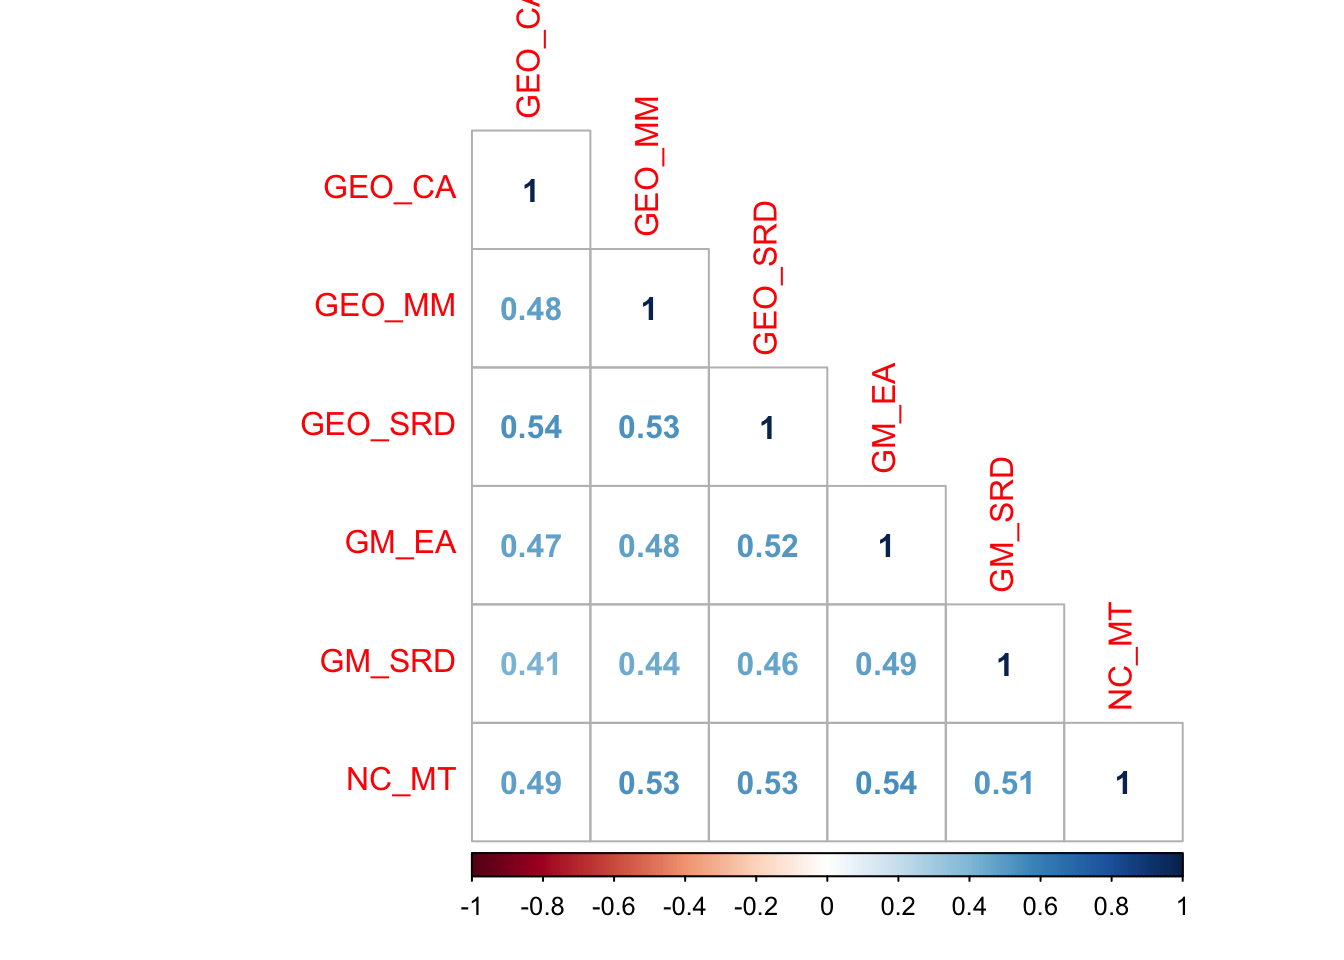
\includegraphics{bookdown-demo_files/figure-latex/mate.gen.cor-1.pdf}

La tabella precedente mostra come i risultati nelle diverse dimensioni siano tra loro correlati. Le correla-zioni tra loro esistenti sono forti. Questo risultato non è inatteso in quanto si tratta di dimensioni parte del costrutto più generale valutato che corrisponde alla matematica in generale. Questa è una giustificazione aggiuntiva alla costruzione della dimensione Matematica generale che rappresentasse il punteggio globa-le del singolo allievo alla prova.

Il quadro generale delle analisi di seguito riportate rispecchia in gran parte il percorso di indagine prodotto nei rapporti precedenti (Crescentini et al., 2014) che ha riguardato le prove standardizzate di matematica e di italiano. Analogamente a quanto fatto allora, in questa sede verranno presentate le analisi descrittive generali dei punteggi ottenuti dagli allievi e le analisi di approfondimento riguardanti i circondari, le classi e gli allievi.

\hypertarget{il-contesto-e-la-scuola}{%
\chapter{Il contesto e la scuola}\label{il-contesto-e-la-scuola}}

\hypertarget{ispettorati}{%
\section{Ispettorati}\label{ispettorati}}

I circondari sono le unità organizzative territoriali più ampie per quanto riguarda le scuole comunali. Il no-stro territorio per quanto riguarda le scuole comunali è diviso in nove aree individuate da un numero cre-scente (attualmente i circondari sono passati da 9 a 7 a causa di una riorganizzazione del sistema, si è preferito però conservare l'organizzazione precedente per coerenza con la raccolta delle informazioni) procedendo da sud verso nord. La popolazione degli allievi che hanno partecipato al test è composta da 2982 bambini (50.8\% maschi e 49.2\% femmine). La ricerca ha coinvolto 193 classi, tra pubbliche (95\%) e private (5\%), di queste 54 sono pluriclassi. Tutti i circondari sono stati testati nel mese di maggio 2014. La distribuzione degli allievi per circondario è rappresentata nel Grafico 3.

\begin{Shaded}
\begin{Highlighting}[]
\NormalTok{joined }\OtherTok{\textless{}{-}} \FunctionTok{read.csv2}\NormalTok{(}\StringTok{"Data/joined.csv"}\NormalTok{) }

\FunctionTok{library}\NormalTok{(ggplot2)}
\FunctionTok{library}\NormalTok{(viridis)}
\FunctionTok{library}\NormalTok{(plotly)}
\FunctionTok{library}\NormalTok{(tidyverse)}


\FunctionTok{table}\NormalTok{(joined}\SpecialCharTok{$}\NormalTok{circondari) }
\end{Highlighting}
\end{Shaded}

\begin{verbatim}
## 
##     Bellinzonese e Tre Valli            Locarnese e Valli 
##                          602                          389 
##                     Luganese Mendrisiotto e Basso Ceresio 
##                         1008                          507
\end{verbatim}

\begin{Shaded}
\begin{Highlighting}[]
\NormalTok{circPlot }\OtherTok{\textless{}{-}} \FunctionTok{ggplot}\NormalTok{(joined, }\FunctionTok{aes}\NormalTok{(circondari)) }\SpecialCharTok{+}
  \FunctionTok{geom\_bar}\NormalTok{(}\FunctionTok{aes}\NormalTok{(}\AttributeTok{fill=}\NormalTok{circondari)) }\SpecialCharTok{+}
  \FunctionTok{scale\_fill\_viridis}\NormalTok{(}\AttributeTok{discrete =} \ConstantTok{TRUE}\NormalTok{, }\AttributeTok{alpha =} \FloatTok{0.6}\NormalTok{) }\SpecialCharTok{+}
  \FunctionTok{ylab}\NormalTok{(}\StringTok{"Effettivi"}\NormalTok{) }\SpecialCharTok{+}
  \FunctionTok{xlab}\NormalTok{(}\StringTok{"Circondari"}\NormalTok{) }\SpecialCharTok{+}
  \FunctionTok{ggtitle}\NormalTok{(}\StringTok{"Numero di studenti nei 4 Ispettorati"}\NormalTok{) }\SpecialCharTok{+}
  \FunctionTok{theme}\NormalTok{(}\AttributeTok{axis.text.x =} \FunctionTok{element\_text}\NormalTok{(}\AttributeTok{angle =} \DecValTok{60}\NormalTok{, }\AttributeTok{vjust =} \DecValTok{1}\NormalTok{, }\AttributeTok{hjust=}\DecValTok{1}\NormalTok{, }\AttributeTok{size =} \DecValTok{8}\NormalTok{)) }

\FunctionTok{ggplotly}\NormalTok{(circPlot)}
\end{Highlighting}
\end{Shaded}

\includegraphics{bookdown-demo_files/figure-latex/ispettorati-1.pdf}

Di seguito (Tabella 2) i punteggi medi nei 9 circondari per la variabile per le diverse sottodimensioni ana-lizzate. Le differenze tra i circondari risultano significative in tutte le dimensioni analizzando l'insieme dei dati tramite l'analisi della varianza. Non è possibile attribuire delle cause specifiche a queste differenze. Vale la pena notare come vi siano delle differenze nelle prestazioni nelle singole dimensioni non omoge-nee (un singolo circondario può avere una prestazione complessivamente elevata in una dimensione e modesta in un'altra).

\begin{Shaded}
\begin{Highlighting}[]
\FunctionTok{library}\NormalTok{(tidyr)}
\FunctionTok{library}\NormalTok{(DT)}

\NormalTok{joined }\SpecialCharTok{\%\textgreater{}\%} \FunctionTok{select}\NormalTok{(circondari,GEO\_CA}\SpecialCharTok{:}\NormalTok{Matematica\_Generale) }\SpecialCharTok{\%\textgreater{}\%}
  \FunctionTok{group\_by}\NormalTok{(circondari) }\SpecialCharTok{\%\textgreater{}\%} 
  \FunctionTok{summarise}\NormalTok{(}\FunctionTok{across}\NormalTok{(GEO\_CA}\SpecialCharTok{:}\NormalTok{Matematica\_Generale, mean, }\AttributeTok{na.rm=}\ConstantTok{TRUE}\NormalTok{)) }\SpecialCharTok{\%\textgreater{}\%}
  \FunctionTok{mutate}\NormalTok{(}\FunctionTok{across}\NormalTok{(GEO\_CA}\SpecialCharTok{:}\NormalTok{Matematica\_Generale, round, }\DecValTok{3}\NormalTok{))  }\SpecialCharTok{\%\textgreater{}\%} 
  \FunctionTok{datatable}\NormalTok{()}
\end{Highlighting}
\end{Shaded}

\includegraphics{bookdown-demo_files/figure-latex/ispettorati_ris-1.pdf}

\begin{Shaded}
\begin{Highlighting}[]
\NormalTok{joined\_long }\OtherTok{\textless{}{-}}\NormalTok{ joined }\SpecialCharTok{\%\textgreater{}\%}
  \FunctionTok{pivot\_longer}\NormalTok{(}\AttributeTok{cols=}\NormalTok{GEO\_CA}\SpecialCharTok{:}\NormalTok{Matematica\_Generale, }\AttributeTok{names\_to =} \StringTok{"Dimensioni"}\NormalTok{, }\AttributeTok{values\_to =} \StringTok{"score"}\NormalTok{)}

\CommentTok{\# plot risultati matematica}

\NormalTok{ris\_medi.circ\_hist }\OtherTok{\textless{}{-}}\NormalTok{ joined\_long }\SpecialCharTok{\%\textgreater{}\%}
  \FunctionTok{ggplot}\NormalTok{(}\FunctionTok{aes}\NormalTok{(}\AttributeTok{x=}\NormalTok{circondari, }\AttributeTok{y=}\NormalTok{score, }\AttributeTok{fill=}\NormalTok{circondari)) }\SpecialCharTok{+}
  \FunctionTok{geom\_bar}\NormalTok{(}\AttributeTok{position =} \StringTok{"dodge"}\NormalTok{, }\AttributeTok{stat =} \StringTok{"summary"}\NormalTok{, }\AttributeTok{fun.y =} \StringTok{"mean"}\NormalTok{) }\SpecialCharTok{+}
  \FunctionTok{facet\_grid}\NormalTok{(}\SpecialCharTok{\textasciitilde{}}\NormalTok{Dimensioni) }\SpecialCharTok{+}
  \FunctionTok{scale\_fill\_viridis}\NormalTok{(}\AttributeTok{discrete =} \ConstantTok{TRUE}\NormalTok{, }\AttributeTok{alpha =} \FloatTok{0.9}\NormalTok{) }\SpecialCharTok{+}
  \FunctionTok{theme}\NormalTok{(}
    \AttributeTok{legend.position=}\StringTok{"none"}\NormalTok{,}
    \AttributeTok{plot.title =} \FunctionTok{element\_text}\NormalTok{(}\AttributeTok{size=}\DecValTok{11}\NormalTok{)}
\NormalTok{  ) }\SpecialCharTok{+}
  \FunctionTok{ggtitle}\NormalTok{(}\StringTok{"Punteggi medi degli allievi nelle diverse dimensioni"}\NormalTok{) }\SpecialCharTok{+}
  \FunctionTok{xlab}\NormalTok{(}\StringTok{""}\NormalTok{) }\SpecialCharTok{+}
  \FunctionTok{theme}\NormalTok{(}\AttributeTok{axis.text.x =} \FunctionTok{element\_text}\NormalTok{(}\AttributeTok{angle =} \DecValTok{60}\NormalTok{, }\AttributeTok{vjust =} \DecValTok{1}\NormalTok{, }\AttributeTok{hjust=}\DecValTok{1}\NormalTok{, }\AttributeTok{size =} \DecValTok{8}\NormalTok{))}
\end{Highlighting}
\end{Shaded}

\begin{verbatim}
## Warning: Ignoring unknown parameters: fun.y
\end{verbatim}

\begin{Shaded}
\begin{Highlighting}[]
\FunctionTok{plot}\NormalTok{(ris\_medi.circ\_hist)}
\end{Highlighting}
\end{Shaded}

\begin{verbatim}
## No summary function supplied, defaulting to `mean_se()`
## No summary function supplied, defaulting to `mean_se()`
## No summary function supplied, defaulting to `mean_se()`
## No summary function supplied, defaulting to `mean_se()`
## No summary function supplied, defaulting to `mean_se()`
## No summary function supplied, defaulting to `mean_se()`
## No summary function supplied, defaulting to `mean_se()`
\end{verbatim}

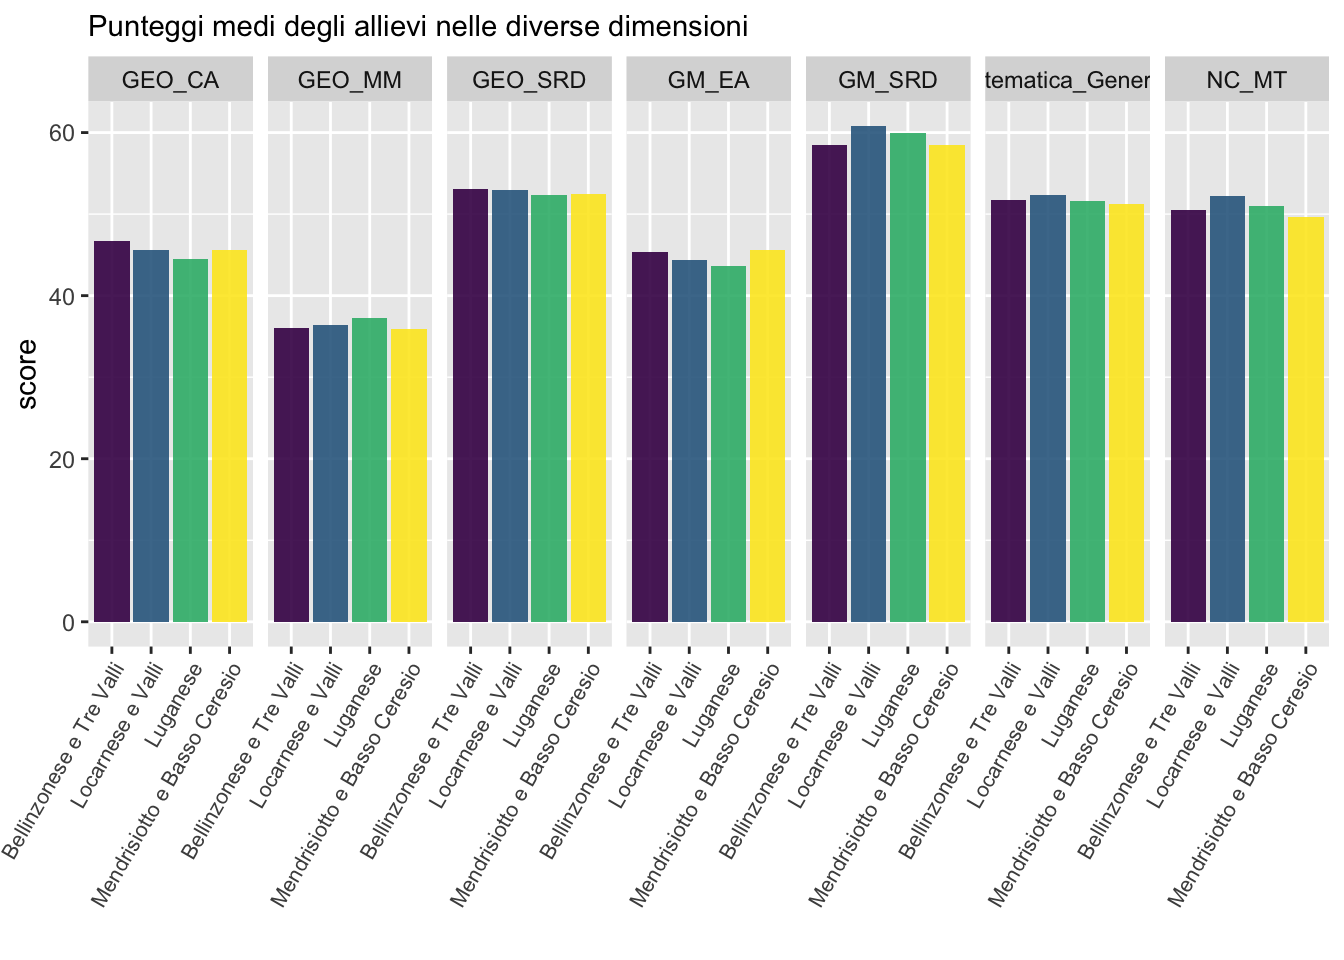
\includegraphics{bookdown-demo_files/figure-latex/ispettorati_ris-2.pdf}

\begin{Shaded}
\begin{Highlighting}[]
\NormalTok{ris\_medi.circ }\OtherTok{\textless{}{-}}\NormalTok{ joined\_long }\SpecialCharTok{\%\textgreater{}\%}
  \FunctionTok{ggplot}\NormalTok{(}\FunctionTok{aes}\NormalTok{(}\AttributeTok{x=}\NormalTok{Dimensioni, }\AttributeTok{y=}\NormalTok{score, }\AttributeTok{fill=}\NormalTok{Dimensioni)) }\SpecialCharTok{+}
  \FunctionTok{geom\_boxplot}\NormalTok{() }\SpecialCharTok{+}
  \FunctionTok{facet\_wrap}\NormalTok{(}\SpecialCharTok{\textasciitilde{}}\NormalTok{circondari) }\SpecialCharTok{+}
  \FunctionTok{scale\_fill\_viridis}\NormalTok{(}\AttributeTok{discrete =} \ConstantTok{TRUE}\NormalTok{, }\AttributeTok{alpha =} \FloatTok{0.6}\NormalTok{) }\SpecialCharTok{+}
  \FunctionTok{theme}\NormalTok{(}
    \AttributeTok{legend.position=}\StringTok{"none"}\NormalTok{,}
    \AttributeTok{plot.title =} \FunctionTok{element\_text}\NormalTok{(}\AttributeTok{size=}\DecValTok{11}\NormalTok{)}
\NormalTok{  ) }\SpecialCharTok{+}
  \FunctionTok{ggtitle}\NormalTok{(}\StringTok{"Punteggi medi degli allievi nelle diverse dimensioni"}\NormalTok{) }\SpecialCharTok{+}
  \FunctionTok{xlab}\NormalTok{(}\StringTok{""}\NormalTok{) }\SpecialCharTok{+}
  \FunctionTok{theme}\NormalTok{(}\AttributeTok{axis.text.x =} \FunctionTok{element\_text}\NormalTok{(}\AttributeTok{angle =} \DecValTok{60}\NormalTok{, }\AttributeTok{vjust =} \DecValTok{1}\NormalTok{, }\AttributeTok{hjust=}\DecValTok{1}\NormalTok{, }\AttributeTok{size =} \DecValTok{8}\NormalTok{))}
\FunctionTok{ggplotly}\NormalTok{(ris\_medi.circ)}
\end{Highlighting}
\end{Shaded}

\begin{verbatim}
## Warning: `group_by_()` was deprecated in dplyr 0.7.0.
## Please use `group_by()` instead.
## See vignette('programming') for more help
## This warning is displayed once every 8 hours.
## Call `lifecycle::last_warnings()` to see where this warning was generated.
\end{verbatim}

\includegraphics{bookdown-demo_files/figure-latex/ispettorati_ris-3.pdf}

\begin{Shaded}
\begin{Highlighting}[]
\NormalTok{ris\_medi.circ2 }\OtherTok{\textless{}{-}}\NormalTok{ joined\_long }\SpecialCharTok{\%\textgreater{}\%}
  \FunctionTok{ggplot}\NormalTok{(}\FunctionTok{aes}\NormalTok{(}\AttributeTok{x=}\NormalTok{circondari, }\AttributeTok{y=}\NormalTok{score, }\AttributeTok{fill=}\NormalTok{circondari)) }\SpecialCharTok{+}
  \FunctionTok{geom\_boxplot}\NormalTok{() }\SpecialCharTok{+}
  \FunctionTok{facet\_wrap}\NormalTok{(}\SpecialCharTok{\textasciitilde{}}\NormalTok{Dimensioni) }\SpecialCharTok{+}
  \FunctionTok{scale\_fill\_viridis}\NormalTok{(}\AttributeTok{discrete =} \ConstantTok{TRUE}\NormalTok{, }\AttributeTok{alpha =} \FloatTok{0.6}\NormalTok{) }\SpecialCharTok{+}
  \FunctionTok{theme}\NormalTok{(}
    \AttributeTok{legend.position=}\StringTok{"none"}\NormalTok{,}
    \AttributeTok{plot.title =} \FunctionTok{element\_text}\NormalTok{(}\AttributeTok{size=}\DecValTok{11}\NormalTok{)}
\NormalTok{  ) }\SpecialCharTok{+}
  \FunctionTok{ggtitle}\NormalTok{(}\StringTok{"Punteggi medi degli allievi nelle diverse dimensioni"}\NormalTok{) }\SpecialCharTok{+}
  \FunctionTok{xlab}\NormalTok{(}\StringTok{""}\NormalTok{) }\SpecialCharTok{+}
  \FunctionTok{theme}\NormalTok{(}\AttributeTok{axis.text.x =} \FunctionTok{element\_text}\NormalTok{(}\AttributeTok{angle =} \DecValTok{60}\NormalTok{, }\AttributeTok{vjust =} \DecValTok{1}\NormalTok{, }\AttributeTok{hjust=}\DecValTok{1}\NormalTok{, }\AttributeTok{size =} \DecValTok{8}\NormalTok{))}
\FunctionTok{ggplotly}\NormalTok{(ris\_medi.circ2)}
\end{Highlighting}
\end{Shaded}

\includegraphics{bookdown-demo_files/figure-latex/ispettorati_ris-4.pdf}

\begin{Shaded}
\begin{Highlighting}[]
\NormalTok{ris\_medi.circ3 }\OtherTok{\textless{}{-}}\NormalTok{ joined\_long }\SpecialCharTok{\%\textgreater{}\%}
  \FunctionTok{ggplot}\NormalTok{(}\FunctionTok{aes}\NormalTok{(}\AttributeTok{x=}\NormalTok{circondari, }\AttributeTok{y=}\NormalTok{score, }\AttributeTok{fill=}\NormalTok{circondari)) }\SpecialCharTok{+}
  \FunctionTok{geom\_boxplot}\NormalTok{() }\SpecialCharTok{+}
  \FunctionTok{facet\_grid}\NormalTok{(}\SpecialCharTok{\textasciitilde{}}\NormalTok{Dimensioni) }\SpecialCharTok{+}
  \FunctionTok{scale\_fill\_viridis}\NormalTok{(}\AttributeTok{discrete =} \ConstantTok{TRUE}\NormalTok{, }\AttributeTok{alpha =} \FloatTok{0.6}\NormalTok{) }\SpecialCharTok{+}
  \FunctionTok{theme}\NormalTok{(}
    \AttributeTok{legend.position=}\StringTok{"none"}\NormalTok{,}
    \AttributeTok{plot.title =} \FunctionTok{element\_text}\NormalTok{(}\AttributeTok{size=}\DecValTok{11}\NormalTok{)}
\NormalTok{  ) }\SpecialCharTok{+}
  \FunctionTok{ggtitle}\NormalTok{(}\StringTok{"Punteggi medi degli allievi nelle diverse dimensioni"}\NormalTok{) }\SpecialCharTok{+}
  \FunctionTok{xlab}\NormalTok{(}\StringTok{""}\NormalTok{) }\SpecialCharTok{+}
  \FunctionTok{theme}\NormalTok{(}\AttributeTok{axis.text.x =} \FunctionTok{element\_text}\NormalTok{(}\AttributeTok{angle =} \DecValTok{60}\NormalTok{, }\AttributeTok{vjust =} \DecValTok{1}\NormalTok{, }\AttributeTok{hjust=}\DecValTok{1}\NormalTok{, }\AttributeTok{size =} \DecValTok{8}\NormalTok{))}
\FunctionTok{ggplotly}\NormalTok{(ris\_medi.circ3)}
\end{Highlighting}
\end{Shaded}

\includegraphics{bookdown-demo_files/figure-latex/ispettorati_ris-5.pdf}

\begin{Shaded}
\begin{Highlighting}[]
\FunctionTok{library}\NormalTok{(apaTables)}
\NormalTok{isp\_aov }\OtherTok{\textless{}{-}} \FunctionTok{aov}\NormalTok{(joined}\SpecialCharTok{$}\NormalTok{Matematica\_Generale }\SpecialCharTok{\textasciitilde{}}\NormalTok{ joined}\SpecialCharTok{$}\NormalTok{circondari, }\AttributeTok{data=}\NormalTok{joined)}

\FunctionTok{apa.1way.table}\NormalTok{(}\AttributeTok{iv =}\NormalTok{ circondari, }\AttributeTok{dv =}\NormalTok{ Matematica\_Generale, }\AttributeTok{data=}\NormalTok{joined)}
\end{Highlighting}
\end{Shaded}

\begin{verbatim}
## 
## 
## Descriptive statistics for Matematica_Generale as a function of circondari.  
## 
##                    circondari     M    SD
##      Bellinzonese e Tre Valli 51.75 13.15
##             Locarnese e Valli 52.31 12.24
##                      Luganese 51.62 14.26
##  Mendrisiotto e Basso Ceresio 51.24 13.57
## 
## Note. M and SD represent mean and standard deviation, respectively.
## 
\end{verbatim}

\begin{Shaded}
\begin{Highlighting}[]
\FunctionTok{apa.aov.table}\NormalTok{(isp\_aov)}
\end{Highlighting}
\end{Shaded}

\begin{verbatim}
## 
## 
## ANOVA results using joined$Matematica_Generale as the dependent variable
##  
## 
##          Predictor         SS   df         MS       F    p partial_eta2
##        (Intercept) 1612359.68    1 1612359.68 8768.75 .000             
##  joined$circondari     256.74    3      85.58    0.47 .706          .00
##              Error  460056.67 2502     183.88                          
##  CI_90_partial_eta2
##                    
##          [.00, .00]
##                    
## 
## Note: Values in square brackets indicate the bounds of the 90% confidence interval for partial eta-squared
\end{verbatim}

Dalle analisi di varianza effettuate emerge come non vi siano differenze statisticamente significative rispetto ai risultati in matematica generale tra i 4 ispettorati del territorio ticinese.

\hypertarget{applications}{%
\chapter{Applications}\label{applications}}

Some \emph{significant} applications are demonstrated in this chapter.

\hypertarget{example-one}{%
\section{Example one}\label{example-one}}

\hypertarget{example-two}{%
\section{Example two}\label{example-two}}

\hypertarget{final-words}{%
\chapter{Final Words}\label{final-words}}

We have finished a nice book.

  \bibliography{book.bib,packages.bib}

\end{document}
